\section{Auswertung}
Die zu Beginn des Versuchs durchgeführte Nullmessung ergibt die in Abbildung $\ref{Leermessung}$ dargestellte Energieverteilung. Sie zeigt deutlich den bei $^{137}$Cs auftretenden Peak um $662 \, \si{\kilo\electronvolt}$ sowie die davor liegende
Compton-Kante. Es werden $11059$ Ereignisse in $60.42 \, \si{\second}$, oder $183 \,  \pm \, 3\, \frac{\text{Zä}}{\si{\second}}$ gemessen.
\begin{figure}[H]
  \centering
  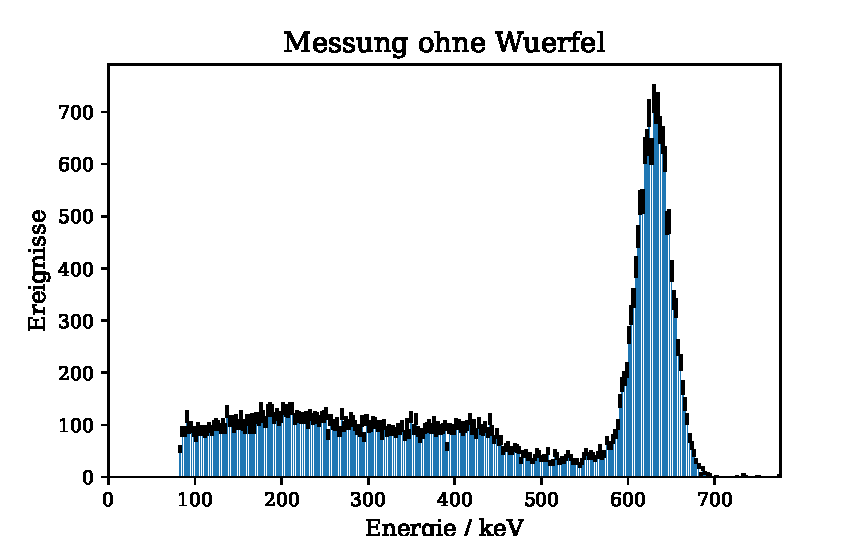
\includegraphics{plots/leer.pdf}
  \caption{Balkendiagramm der Leermessung.}
  \label{Leermessung}
\end{figure}
\subsection{Leerer Würfel}
Der Intensitätsvektor für die verschiedenen Projektionen der ersten Messung ist in $\ref{eq:vecleer1}$ zu finden, die der zweiten in $\ref{eq:vecleer2}$.
Aufgrund des homogenen Aufbaus des Würfels,
werden für nicht vermessene Projektionsrichtungen die Werte von äquivalenten Projektionen eingesetzt.
Vermessen werden die Projektionsrichtungen 1, 3, 10, 11 und 12. Die Angegebenen Fehler ergeben sich aus dem Fehler der gemessenen Ereignisse geteilt durch die Zeit. Es ist
zu Erwähnen, dass zwischen den beiden Messungen die Würfel 2 und 3 Untersucht wurden um die Messung auf systematische Fehler zu prüfen.

\begin{equation}
	\vec{I_1}=
	\begin{pmatrix}
		\num{180.1 \pm 2.4} \\
		\num{180.1 \pm 2.4} \\
		\num{180.1\pm 2.4} \\
		\num{178.8\pm 2.4} \\
		\num{178.8\pm 2.4} \\
		\num{178.8\pm 2.4} \\
		\num{176.6\pm 2.4} \\
		\num{177.0\pm 2.4} \\
		\num{175.9\pm 2.4} \\
    \num{176.6\pm 2.4} \\
    \num{177.0\pm 2.4} \\
    \num{175.9\pm 2.4} \\
	\end{pmatrix}
    \sfrac{\text{counts}}{\text{s}}
	\label{eq:vecleer1}
\end{equation}
\begin{equation}
	\vec{I_2}=
	\begin{pmatrix}
		\num{171.7 \pm 2.5} \\
		\num{171.7 \pm 2.5} \\
		\num{171.7\pm 2.5} \\
		\num{173.3\pm 2.4} \\
		\num{173.3\pm 2.4} \\
		\num{173.3\pm 2.4} \\
		\num{165.2\pm 2.5} \\
		\num{161.8\pm 2.5} \\
		\num{174.1\pm 1.9} \\
    \num{165.2\pm 2.5} \\
    \num{162.8\pm 2.5} \\
    \num{174.1\pm 1.9} \\
	\end{pmatrix}
    \sfrac{\text{counts}}{\text{s}}
	\label{eq:vecleer2}
\end{equation}
Es ist festzustellen, dass zwischen den beiden Messungen zum Teil Abweichungen außerhalb der Messungenauigkeit auftreten. Eine Erklärung für diese Abweichungen könnte sein, dass die Messapparaturen erst mit der Zeit warmlaufen müssen.
\subsection{Untersuchung der Würfel 2 und 3}
Die Bestimmung des Absorptionskoeffizienten der Würfel 2 und 3, welche jeweils komplett aus Aluminium oder Blei bestehen, nutzt die Tatsache, dass sich durch deren Aufbau die verschiedenen gemessenen Projektionen mitteln lassen
und es möglich ist, die Geometriematrix zu einem Vektor in den einzelnen Komponenten zu summieren. Diese Vektoren $\vec{A_2}$ und $\vec{A_3}$ sind:
\begin{equation}
	\vec{A_2}=
	\begin{pmatrix}
		2\sqrt{2} \\
		3\sqrt{2} \\
		2\sqrt{2} \\
		\sqrt{2}\\
    \sqrt{2}
	\end{pmatrix}
\end{equation}
\begin{equation}
	\vec{A_3}=
	\begin{pmatrix}
		2\sqrt{2} \\
		3\sqrt{2} \\
		2\sqrt{2} \\
		\sqrt{2}\\
	\end{pmatrix}
\end{equation}
Als Intensitätsvektoren ergeben sich:
\begin{equation}
	\vec{I_{Alu}}=
	\begin{pmatrix}
		\num{93.9 \pm 2.5} \\
		\num{93.9 \pm 2.5} \\
		\num{93.9\pm 2.5} \\
		\num{97.6\pm 2.5} \\
		\num{97.6\pm 2.5} \\
		\num{97.6\pm 2.5} \\
		\num{88.2\pm 2.4} \\
		\num{84.3\pm 2.5} \\
		\num{110.1\pm 2.4} \\
    \num{88.2\pm 2.4} \\
    \num{84.3\pm 2.5} \\
    \num{110.1\pm 2.4} \\
	\end{pmatrix}
    \sfrac{\text{counts}}{\text{s}}
	\label{eq:vecleer1}
\end{equation}
\begin{equation}
	\vec{I_{Blei}}=
	\begin{pmatrix}
		\num{5.6 \pm 0.3} \\
		\num{5.6 \pm 0.3} \\
		\num{5.6\pm 0.3} \\
		\num{5.6\pm 0.3} \\
		\num{5.6\pm 0.3} \\
		\num{5.6\pm 0.3} \\
		\num{3.8\pm 0.2} \\
		\num{3.0\pm 0.2} \\
		\num{5.0\pm 0.2} \\
    \num{3.8\pm 0.2 } \\
    \num{3.0\pm 0.2} \\
    \num{5.0\pm 0.2} \\
	\end{pmatrix}
    \sfrac{\text{counts}}{\text{s}}
	\label{eq:vecleer1}
\end{equation}
Die Fehler werden hier wie beim leeren Würfel ermittelt.
$\vec{A_2}$ und $\vec{A_3}$ erlauben es, mit einen Least-Square-Fit und Gleichung $\ref{eq:abweichung}$, die Absorptionskoeffizienten zu berechnen.
Zur Berücksichtigung des Würfelgehäuses wird hierbei $\vec{I_1}$ genutzt.
\clearpage
Es ergibt sich:
\begin{table}[H]
  \centering
\begin{tabular}{c|c|c}
  & Material &  $\mu,\frac{1}{\si{cm}}$ \\
  \hline
Würfel 2 & Aluminium & $0.22 \pm 0.02$ \\
Würfel 3 & Blei      & $1.26 \pm 0.09$
\end{tabular}
\end{table}
Für Würfel 2 werden bei der Untersuchung die Projektionsrichtungen 1, 3, 10, 11, 12 und bei Würfel 3: 3, 10, 11, 12 genommen.
\subsection{Untersuchung von Würfel 5}
Der Würfel unbekannten Aufbaus (Würfel 5) wird mit zwölf Projektionsrichtungen untersucht, um Rückschlüsse auf das Material der einzelnen Elementarwürfel zu erlauben.
Die Projektionsrichtungen sind durch die Matrix \ref{eq:gigamatrix} gegeben.
Da die Materialzusammensetzung des Würfels gänzlich unbekannt ist, ist es in diesem Fall nicht möglich die Geometriematrix A zu vereinfachen.
Die Einträge der Matrix ergeben sich aus 0, wenn die Richtung nicht durchlaufen wird,
 aus 1, wenn der Würfel mit einer Kantenlänge durchlaufen wird und mit $\sqrt{2}$ für ein Durchlaufen durch eine Diagonale.
\begin{equation}
	A=
	\begin{pmatrix}
    1& 1& 1& 0& 0& 0& 0& 0& 0\\
    0& 0& 0& 1& 1& 1& 0& 0& 0\\
    0 & 0& 0& 0& 0& 0& 1& 1& 1\\
    1& 0& 0& 1& 0& 0& 1& 0& 0\\
    0& 1& 0& 0& 1& 0& 0& 1& 0\\
    0& 0& 1& 0& 0& 1& 0& 0& 1\\
    0& \sqrt{2}& 0& \sqrt{2}& 0& 0& 0& 0& 0\\
    0& 0& \sqrt{2}& 0&\sqrt{2}& 0& \sqrt{2}& 0& 0\\
    0& 0& 0& 0& 0&\sqrt{2}& 0& \sqrt{2}& 0\\
    0& 0& 0&\sqrt{2}& 0& 0& 0&\sqrt{2}& 0\\
    \sqrt{2}& 0& 0& 0& \sqrt{2}& 0& 0& 0& \sqrt{2}\\
    0& \sqrt{2}& 0& 0& 0& \sqrt{2}& 0& 0& 0
	\end{pmatrix}
  \label{eq:gigamatrix}
\end{equation}
Der Intensitätsvektor $\vec{I_5}$ und der Logarithmus von $\vec{I_5}$ ($\vec{\tilde{I_5}}$) lauten:
\begin{equation}
	\vec{I_5}=
	\begin{pmatrix}
		\num{35.9 \pm 1.2} \\
		\num{35.3 \pm 1.2} \\
		\num{88.3\pm 1.9} \\
		\num{84.2\pm 1.8} \\
		\num{34.1\pm 1.1} \\
		\num{72.2\pm 1.7} \\
		\num{85.5\pm 1.7} \\
		\num{28.2\pm 1.0} \\
		\num{25.1\pm 1.0} \\
    \num{103.5\pm 1.9} \\
    \num{39.3\pm 1.2} \\
    \num{24.5\pm 0.9} \\
	\end{pmatrix}
    \sfrac{\text{counts}}{\text{s}}
	\label{eq:vec5}
\end{equation}
\begin{equation}
	\vec{\tilde{I_5}}=
	\begin{pmatrix}
		\num{1.6 \pm 0.2} \\
		\num{1.6 \pm 0.2} \\
		\num{0.7\pm 0.1} \\
		\num{0.7\pm 0.1} \\
		\num{1.6\pm 0.2} \\
		\num{0.9\pm 0.1} \\
		\num{0.7\pm 0.1} \\
		\num{1.8\pm 0.2} \\
		\num{1.9\pm 0.2} \\
    \num{0.5\pm 0.1} \\
    \num{1.5\pm 0.2} \\
    \num{2.0\pm 0.2} \\
	\end{pmatrix}
    \sfrac{\text{counts}}{\text{s}}
	\label{eq:vec6}
\end{equation}
Die angegeben Fehler werden hierbei erneut durch den Fehler der gemessenen Ereignisse geteilt durch die Messdauer bestimmt.
Die Absorptionskoeffizienten $\mu$ der Teilwürfel lassen sich hiermit wie bei den Würfeln 2 und 3 bestimmen.\\
Es ergibt sich:
\begin{table}[H]
\centering
\caption{Berechnete Absorptionskoeffizienten der einzelnen Teilwürfel.}
\label{companioncube}
\begin{tabular}{c|c|c|c}
  Elementarwürfel& $\mu$ in $\frac{1}{\si{cm}}$& Zugeordnetes Material & Abweichung in \%\\
  \hline
1 & 0.56 \pm \, 0.09 & Eisen & 2.4\\
2 & 0.6  \pm \, 0.07&Messing & 2.2\\
3 & 0.29 \pm\, 0.1  &Aluminium & 42.9\\
4 & -0.1  \pm\, 0.06&Delrin & 186.2\\
5 & 0.69 \pm \,0.08 &Messing & 12.4\\
6 & 0.86  \pm \,0.08& Messing & 40.1\\
7 & 0.33  \pm \, 0.08& Aluminium & 62.6\\
8 & 0.49  \pm \,0.07 &Eisen & 14.6\\
9 & -0.19 \pm \,0.09 &Delrin & 263.8\\
\end{tabular}
\end{table}
Hierbei wurden den Elementarwürfeln jeweils das Material mit der kleinsten Abweichung zugeordnet. Die zur bestimmung genutzten Literaturwerte finden sich in Tabelle 2.
